\documentclass{article}

\usepackage[left=2cm,right=2cm,top=2cm,bottom=2cm]{geometry} 

\usepackage[utf8]{inputenc}   % otra alternativa para los caracteres acentuados y la "ñ"
\usepackage[           spanish % para poder usar el español
                      ,es-tabla % para los captions de las tablas
                       ]{babel}   
\decimalpoint %para usar el punto decimal en vez de coma para los números con decimales

%\usepackage{beton}
%\usepackage[T1]{fontenc}

\usepackage{parskip}
\usepackage{xcolor}

\usepackage{caption}

\usepackage{enumerate} % paquete para poder personalizar fácilmente la apariencia de las listas enumerativas

\usepackage{graphicx} % figuras
\usepackage{subfigure} % subfiguras

\usepackage{amsfonts}
\usepackage{amsmath}

\usepackage{listings}
\lstset
{ %Formatting for code in appendix
    language=python,
    basicstyle=\footnotesize,
    stepnumber=1,
    showstringspaces=false,
    tabsize=1,
    breaklines=true,
    breakatwhitespace=false,
}

\definecolor{gris}{RGB}{220,220,220}
	
\usepackage{float} % para controlar la situación de los entornos flotantes

\restylefloat{figure}
\restylefloat{table} 
\setlength{\parindent}{0mm}


\usepackage[bookmarks=true,
            bookmarksnumbered=false, % true means bookmarks in 
                                     % left window are numbered
            bookmarksopen=false,     % true means only level 1
                                     % are displayed.
            colorlinks=true,
            allcolors=blue,
            urlcolor=blue]{hyperref}
\definecolor{webblue}{rgb}{0, 0, 0.5}  % less intense blue

\usepackage[ruled,vlined]{algorithm2e}
\SetKwInOut{Parameter}{parameter}
\newcommand{\Or}{\textbf{ or }}
\renewcommand{\And}{\textbf{ and }}


\title{\Huge Metaheurística: Práctica Alternativa al Examen \\ Búsqueda Ramificada con Momentos \vspace{10mm}}

\author{\huge David Cabezas Berrido \vspace{10mm} \\
	\huge 20079906D \vspace{10mm} \\  
  \huge Grupo 2: Viernes \vspace{10mm} \\ 
  \huge dxabezas@correo.ugr.es \vspace{10mm}}

\begin{document}
\maketitle
\newpage
\tableofcontents
\newpage

\section{Descripción de la Metaheurística}

Nuestro problema es la optimización continua de una serie de funciones. Estamos limitados por el número de evaluaciones, que en nuestro
caso será 10000 multiplicado por la dimensión del espacio de soluciones.

Diseñaremos nuestra propia metaheurística y la pondremos a prueba con el benchmark CEC'2017. Por tanto, nuestro objetivo es la optimización de parámetros
reales. Con nuestra propuesta esperamos alcanzar un buen compromiso entre exploración y explotación aprovechando la naturaleza continua del espacio
de soluciones.

\subsection{Idea general}
Nuestra metaheurística, \textbf{Búsqueda Ramificada con Momentos}, pretende ``lanzar'' soluciones que se muevan por el espacio como lo harían bombas
lanzadas desde un avión bombardeos, fragmentos que se desprenden de un cuerpo celeste o el despliegue de una sonda de una nave espacial.
Es decir, se explora el espacio ramificando o dividiendo las soluciones en otras, de
forma que las soluciones resultantes conserven la inercia de la solución de la que partieron.

\begin{figure}[H]
	\centering
	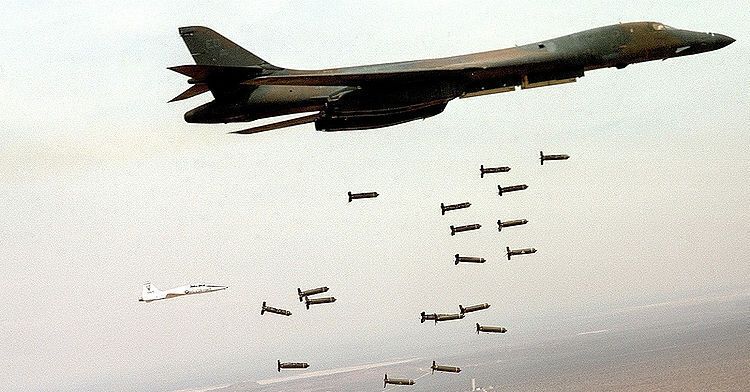
\includegraphics[width=140mm]{imgs/bombs}
	\caption{Cuando se despliegan bombas desde un avión, las bombas mantienen la inercia del movimiento del avión.}
\end{figure}

Para dar sentido a este fenómeno físico que es la conservación de la inercia ideamos una estrategia de explotación basada en momentos, similar
a la Búsqueda Local salvo que se pondera el momento de la solución con la dirección de un vecino mejor.

Las soluciones pueden ser truncadas bajo ciertas
condiciones, así que se van lanzando nuevas soluciones desde puntos aleatorios hasta agotar el número máximo de evaluaciones.

\subsection{Explicación del algoritmo}

El algoritmo comienza con una solución aleatoria, un vector aleatorio de flotantes, $S$. Cada solución tiene asociado otro vector aleatorio que es
su momento, $\nu$, que intuitivamente se puede interpretar como la dirección en la que se está moviendo la solución actualmente; también tiene un
valor escalar positivo, $\lambda$ que podría interpretarse como un impulso, la solución se desplaza usando su momento y su impulso:
$S\gets S+\lambda\nu$.

Cada solución tiene un número determinado de evaluaciones. En cada iteración, una solución puede hacer una de las siguientes acciones:
\begin{itemize}
	\item La solución desaparece, es truncada.
	\item La solución se divide en dos, que ``saldrán disparadas'' en direcciones opuestas.
	\item La solución desvía su dirección hacia un vecino del entorno con mejor fitness y luego se actualiza usando su impulso y su momento: $S\gets S+\lambda\nu$. La solución pierde una cantidad de impulso determinada por el éxito de la búsqueda de un vecino mejor en el entorno.
\end{itemize}
La acción a realizar en cada momento depende de la fitness de la solución respecto a la mejor fitness encontrada hasta el momento, del número de evaluaciones restantes y del impulso que le quede a la solución. Queremos truncar soluciones que no tengan muchas posibilidades de mejorar, ya sea porque
estén muy lejos de la mejor hasta el momento y les queden pocas iteraciones o porque su impulso sea prácticamente nulo. Queremos dividir soluciones
que sean de las mejores, tengan bastantes evaluaciones por delante y no acaben de ser lanzadas desde otras, para evitar que haya soluciones muy
cercanas entre sí.

Estos objetivos pueden ser muy difíciles de lograr debido al número de factores a tener en cuenta, a continuación presentamos nuestro intento de
lograr un equilibrio.

\subsubsection*{Decisión de la acción}

En nuestro caso, primero tomaremos la diferencia entre la fitness de la solución y la mejor fitness encontrada hasta el momento: $D\gets fitness-best$.
Como estamos minimizando, será una cantidad no negativa. En principio tenemos $D\in[0,+\infty[$, para normalizar la escala utilizamos una función
creciente que identifique este intervalo con el $[0,1[$, $\hat{D}\gets \dfrac{D}{1+D}$.

Decidimos truncar la solución cuando esta diferencia sea alta y
las posibilidades de mejorarla sean escasas, ya sea por que la solución tenga pocas evaluaciones restantes o porque su impulso sea bajo.

Decidimos ramificar la solución en dos cuando esta diferencia sea baja, el impulso esté en un rango determinado (no queremos dividir ni muy pronto ni
muy tarde) y el número de evaluaciones restantes sea suficiente para que las soluciones resultantes puedan mejorar.

En el resto de casos, la solución se limita a avanzar.

En nuestra implementación, hemos decidido dar esta estructura al bucle principal, que combina las ideas anteriores con una componente aleatoria.

 \begin{algorithm}[H]
	\DontPrintSemicolon % Some LaTeX compilers require you to use \dontprintsemicolon instead
	\KwIn{Una solución: vector de flotantes $S$}
	\KwIn{Su momento: vector de flotantes $\mu$}
	\KwIn{Su impulso: escalar positivo $\lambda$}
	\KwIn{Evaluaciones a realizar: entero positivo $evals$}
	$fitness\gets \operatorname{eval}(S)$ \tcp*{Supondremos la función de evaluación siempre disponible}
	$evals\gets evals-1$\;
	$best\gets\operatorname{min}(best, fitness)$\;
	\While{$evals>0$}{
		$D\gets fitness-best$ \tcp*{Suponemos accesible la mejor fitness obtenida hasta el momento}
		$\hat{D}\gets \frac{D}{1+D}$ \tcp*{Diferencia normalizada en $[0,1[$}
		$p\gets U[0,1]$ \tcp*{Flotante aleatorio en $[0,1]$, elegido según la distribución uniforme}
		\If{$(p<P_{vanish}\frac{\hat{D}}{\lambda} \And evals\leq MaxEvalsTruncate) \Or \lambda < MinImpulse$}{
			\text{La solución es truncada.}
		}
		\ElseIf{$p>P_{split}\frac{\hat{D}}{\lambda} \And MinImpulseSplit\leq\lambda\leq MaxImpulseSplit \And evals\geq MinEvalsSplit$}{
			\text{La solución se divide en dos.}
		}
		\Else{La solución avanza.}
	}
	\caption{{\sc Branch:} Búsqueda Ramificada: Bucle Principal.}
	\label{alg:branch}
\end{algorithm}

Más adelante discutiremos los parámetros que han aparecido a lo largo del algoritmo. De momento nos centraremos en detallar cada una de las
acciones que aparecen en el bucle.

\subsubsection*{Truncamiento de la solución}
Cuando una solución es truncada, simplemente se corta el bucle con la orden \textbf{break}. Antes, hay que acumular las evaluaciones a
realizar para que no se desperdicien, las llamadas restantes se acumulan para mejorar futuras soluciones: $spareEvals\gets spareEvals+evals$.

\subsubsection*{Ramificación de la solución}

Cuando una solución se ramifica, se generan dos soluciones con empujes opuestos desde ella y se acumulan los momentos. Además, se
recargan en cierta proporción del impulso perdido desde el inicial, $\lambda_0$. Las evaluaciones pendientes se reparten equitativamente
entre las dos soluciones generadas, como la división es entera, se rescata la evaluación sobrante en caso de que el número de evaluaciones
sea impar. La solución es destruida, ya que se queda sin evaluaciones.

 \begin{algorithm}[H]
	\DontPrintSemicolon % Some LaTeX compilers require you to use \dontprintsemicolon instead
	$modification\gets\text{vector aleatorio, las componentes se generan con una $U[0,1]$}$\;
	$\mu_1\gets \mu + modification$ \tcp*{Las soluciones salen en direcciones opuestas}
	$\mu_2\gets \mu - modification$\;
	$\lambda_1\gets \lambda+SplitImpulse\cdot(\lambda_0-\lambda)$ \tcp*{Se recarga parcialmente el impulso}
	$\lambda_2\gets \lambda+SplitImpulse\cdot(\lambda_0-\lambda)$\;
	$S_1 \gets S+\lambda_1 \mu_1$\;
	$S_2 \gets S+\lambda_2 \mu_2$\;
	$\operatorname{clip}(S_1)$ \tcp*{Si alguna componente se sale del rango, se fija en el borde}
	$\operatorname{clip}(S_2)$\;
	\If{$evals \% 2 = 1$}{
		$spareEvals\gets spareEvals+1$ \tcp*{Para evitar perder evaluaciones}
	}
	$\operatorname{branch}(S_1, \mu_1, \lambda_1, evals/2)$\;
	$\operatorname{branch}(S_2, \mu_2, \lambda_2, evals/2)$\;
	\textbf{break} \tcp*{Esta solución desaparece}
	\caption{{\sc Split:} Ramificación de una solución $S$ como la de entrada del Algoritmo \ref{alg:branch}.}
	\label{alg:split}
\end{algorithm}

\subsubsection*{Avance de la solución}
Para el avance de la solución se buscan vecinos aleatorios en un entorno de la solución, para mí siempre se tiene $\lambda\in]0,1]$ y he escogido radio $\sqrt{\lambda}$. Si se encuentra un vecino mejor en un determinado número de intentos, se considera un éxito y se
modifica el momento de la solución desviándolo hacia la dirección del vecino, la medida en la que se desvía depende de la mejora que
aporte; después se desplaza la solución usando el momento y el impulso y se reduce el impulso ligeramente. Si se fracasa al encontrar
un vecino mejor (se agotan los intentos) interpretamos que estamos en un máximo local (o se acabaron las evaluaciones) y se reduce más
severamente el impulso.

 \begin{algorithm}[H]
	\DontPrintSemicolon % Some LaTeX compilers require you to use \dontprintsemicolon instead
	\While{no se encuentre un vecino mejor\And no se excedan $ImproveLimit$ intentos\And $evals>0$}
	{
		$modification\gets\text{vector aleatorio, las componentes se generan con una $U[-\sqrt{\lambda},\sqrt{\lambda}]$}$\;
		$S'\gets S+modification$ \tcp*{Vecino aleatorio}
		$\operatorname{clip}(S')$\;
		$neighbor\_fitness\gets \operatorname{eval}(S')$\;
		$evals\gets evals-1$\;
	}
	\If{el vecino $S'$ mejora la fitness de $S$}{
		$best\gets\operatorname{min}(best, neighbor\_fitness)$\;
		$D\gets fitness - neighbor\_fitness$\;
		$\hat{D}\gets \frac{D}{1+D}$ \tcp*{Mejora normalizada en $[0,1[$}
		$neighbor\_weight\gets BaseWeight+(1-BaseWeight)\cdot \hat{D}$\;
		$\mu\gets(1-neighbor\_weight)\mu+neighbor\_weight\cdot modification$ \tcp*{Se desvía la inercia de la solución hacia el vecino mejor}
		$S\gets S+\lambda\mu$\tcp*{La solución se desplaza en su dirección}
		$\operatorname{clip}(S)$\;
		$fitness\gets \operatorname{eval}(S)$\;
		$evals\gets evals-1$\;
		$best\gets\operatorname{min}(best, fitness)$\;
		$\lambda\gets DecreaseSuccess\cdot \lambda$ \tcp*{Éxito: se reduce ligeramente el impulso}
	}
	\Else{$\lambda\gets DecreaseFail\cdot \lambda$\tcp*{Fracaso: se reduce severamente el impulso}}
	\caption{{\sc Advance:} Avance de la solución $S$ (la de entrada del Algoritmo \ref{alg:branch}).}
	\label{alg:advance}
\end{algorithm}

\subsubsection*{Invocación del algoritmo}

Para aprovechar las evaluaciones de las soluciones que son truncadas se vuelven a lanzar nuevas soluciones.
Cada ejecución parte de una solución aleatoria con momento aleatorio y un impulso inicial $\lambda_0$.

\begin{algorithm}[H]
	\DontPrintSemicolon % Some LaTeX compilers require you to use \dontprintsemicolon instead
	$best\gets\text{un valor mayor que cualquiera que vaya a aparecer al evaluar posteriormente}$\;
	$spareEvals\gets 10000\cdot\text{dimensión del espacio de soluciones}$\;
	\While{$spareEvals>0$}{
		$evals\gets spareEvals$\;
		$spareEvals\gets 0$\;
		$S\gets\text{vector solución aleatorio, componentes generadas de forma uniforme en el rango: $U[-100,100]$}$\;
		$\mu\gets\text{vector momento aleatorio, componentes generadas con $U[-1,1]$}$\;
		$\operatorname{branch}(S, \mu, \lambda_0, evals)$ \tcp*{$spareEvals$ puede verse incrementada durante la ejecución}
	}
	\caption{{\sc Main:} Llamadas sucesivas al algoritmo de búsqueda Ramificada con Momentos hasta consumir todas las evaluaciones
		disponibles.}
	\label{alg:main}
\end{algorithm}

\section{Implementación y benchmark}

\subsection{Detalles de implementación}

Como hemos comentado, nuestra explicación de la metaheurística es una forma de implementar las ideas que hemos ido comentando.
Probablemente existan mejores alternativas para tomar las decisiones del Algoritmo \ref{alg:branch}, que se basen en las mismas
ideas intuitivas que hemos comentado. Como otro ejemplo, la división de la solución podría ser en más de dos soluciones.

Además, fijada una implementación concreta (la que acabamos de describir), quedan por discutir un gran número de parámetros
que han ido apareciendo a lo largo de la explicación del algoritmo. A continuación presentamos una tabla con los distintos
parámetros, su papel en la metaheurística y el valor concreto que les damos en la ejecución.

\textbf{Nota:} Todos los parámetros toman valores positivos por naturaleza.

\begin{table}[H]
	\centering
	\begin{tabular}{|l|l|l|c|}
		\hline
		\textbf{Parámetro} & \textbf{Tipo / Rango} & \textbf{Papel} & \textbf{Valor} \\ \hline
	$\lambda_0$ & Real & Impulso inicial de las soluciones de partida & 1 \\ \hline
	$MaxEvalsTruncate$ & Entero menor que $10000\cdot\text{dim}$ &  \begin{tabular}{l}Máximo de evaluaciones restantes con \\ las que una solución puede ser truncada\end{tabular}  &  $1200\cdot\text{dim}$   \\ \hline
	$MinImpulse$ & Real menor que $\lambda_0$ & \begin{tabular}{l}Impulso por debajo del cual \\ la solución es truncada\end{tabular} & $0.01\cdot\lambda_0$  \\ \hline
	$MinImpulseSplit$&  Real menor que $\lambda_0$   & \begin{tabular}{l}Mínimo impulso con el que una solución \\ se puede ramificar\end{tabular} &  $0.1\cdot\lambda_0$  \\ \hline
	$MaxImpulseSplit$	& Real en $]MinImpulseSplit,\lambda_0[$  &  \begin{tabular}{l}Máximo impulso con el que una solución \\ se puede ramificar\end{tabular}  &  $0.7\cdot\lambda_0$  \\ \hline
	$MinEvalsSplit$	& Entero menor que $10000\cdot\text{dim}$  &  \begin{tabular}{l}Mínimo de evaluaciones restantes \\ para dividir la solución\end{tabular} &  $400\cdot\text{dim}$              \\ \hline
	$SplitImpulse$	&  Proporción (real en [0,1]) & \begin{tabular}{l}Proporción del impulso perdido que recuperan \\ las soluciones que surgen de una división\end{tabular} &  0.5   \\ \hline
	$ImproveLimit$ & Entero menor que $10000\cdot\text{dim}$ & \begin{tabular}{l}Máximo de intentos para encontrar \\ un vecino mejor\end{tabular} & $10\cdot\text{dim}$ \\ \hline
	$BaseWeight$ & Proporción en $[0,1[$ & \begin{tabular}{l}Mínimo peso en el momento \\ para el vecino que mejora\end{tabular} & 0.2 \\ \hline
	$DecreaseSuccess$ & Proporción en $]0,1[$ & Reducción del impulso en caso de acierto & 0.99 \\ \hline
	$DecreaseFail$ & \begin{tabular}{l} Proporción en \\ $]0,DecreaseSuccess[$\end{tabular} & Reducción del impulso en caso de fallo &  0.9 \\ \hline
	\end{tabular}
	\caption{Tabla con los parámetros del modelo y sus valores concretos en la ejecución.}
	\label{tab:parametros}
\end{table}

Basamos estas elecciones únicamente en nuestra intuición y en el comportamiento del algoritmo (número de veces
que hace cada acción y en qué orden, y valores de las variables, no en los resultados) sobre la función 4 del benchmark en dimensión 10. De modo que seguramente habrá mejores valores para estos parámetros.

\end{document}
